\documentclass[UTF8]{ctexart}

\usepackage{amsmath}
\usepackage{multicol}
\setlength{\parindent}{2em}
\addtolength{\topmargin}{-54pt}
\setlength{\oddsidemargin}{0.63cm}  % 3.17cm - 1 inch
\setlength{\evensidemargin}{\oddsidemargin}
\setlength{\textwidth}{16cm}
\setlength{\textheight}{24.00cm}    % 24.62
\usepackage{graphicx}
\usepackage{float}
\usepackage{multirow}
\usepackage{subfigure}
\usepackage{wrapfig}
\begin{document}

%标题
\begin{center}
\Huge\textbf{高温超导}
\renewcommand{\baselinestretch}{5.0}
\end{center}
\begin{center}
\small
\begin{tabular}{llll}
\textbf{姓名}&李励玮     &\textbf{学号}  &201711140236\\
\textbf{指导老师}&熊俊 &\textbf{实验日期}& 2019.11.1\\
\end{tabular}
\end{center}

\small
\noindent\textbf{摘要}:本实验在低温条件下测量了高温超导体的电阻温度曲线,并与比较了三种低温温度计的电阻温度效应。学习、测量、观察了高临界温度超导体的零电阻现象、迈斯纳效应;测量了金属和半导体的电阻随温度的变化及温差电效应,掌握液氮低温技术。 
\newline\textbf{关键字:零电阻现象;迈斯纳效应;实用超导体;金属、半导体、超导体电阻温度特性}


\begin{multicols}{2}
\section{引言}
当温度低于某一温度时,超导体的电阻突然跌落到零,这就是零电阻现象或超导电现象。超导体内磁场保持不变为零,这是迈斯纳效应。完全导电性和完全抗磁性是超导体的两个基本特性。BCS理论可以解释常规超导体的超导电性。YBCO是目前最流行的高温超导材料,超导电性可以应用于例如超导磁悬浮列车、超导重力仪、超导计算机、超导做波器件等器件。

\section{实验目的}
1.通过对高温超导材料的检测和演示,加深对零电阻现象和迈斯纳效应的理解。

2.了解金属和半导体的电阻随温度变化以及温差电效应。

3.了解超导磁悬浮原理。

4.掌握液氮低温技术。

\section{实验原理}

\subsection{超导现象、临界参数及实用超导体}

\subsubsection{零电阻现象}
当温度低于某一温度时,超导体的电阻突然跌落到零,这就是零电阻现象或超导电现象。

理论上,超导临界温度的定义为:当电流、磁场及其它外部条件(如应力、辐照)保持为零或不影响转变温度测量的足够低值时,超导
体呈现超导态的最高温度。
\begin{figure}[H]
\centering
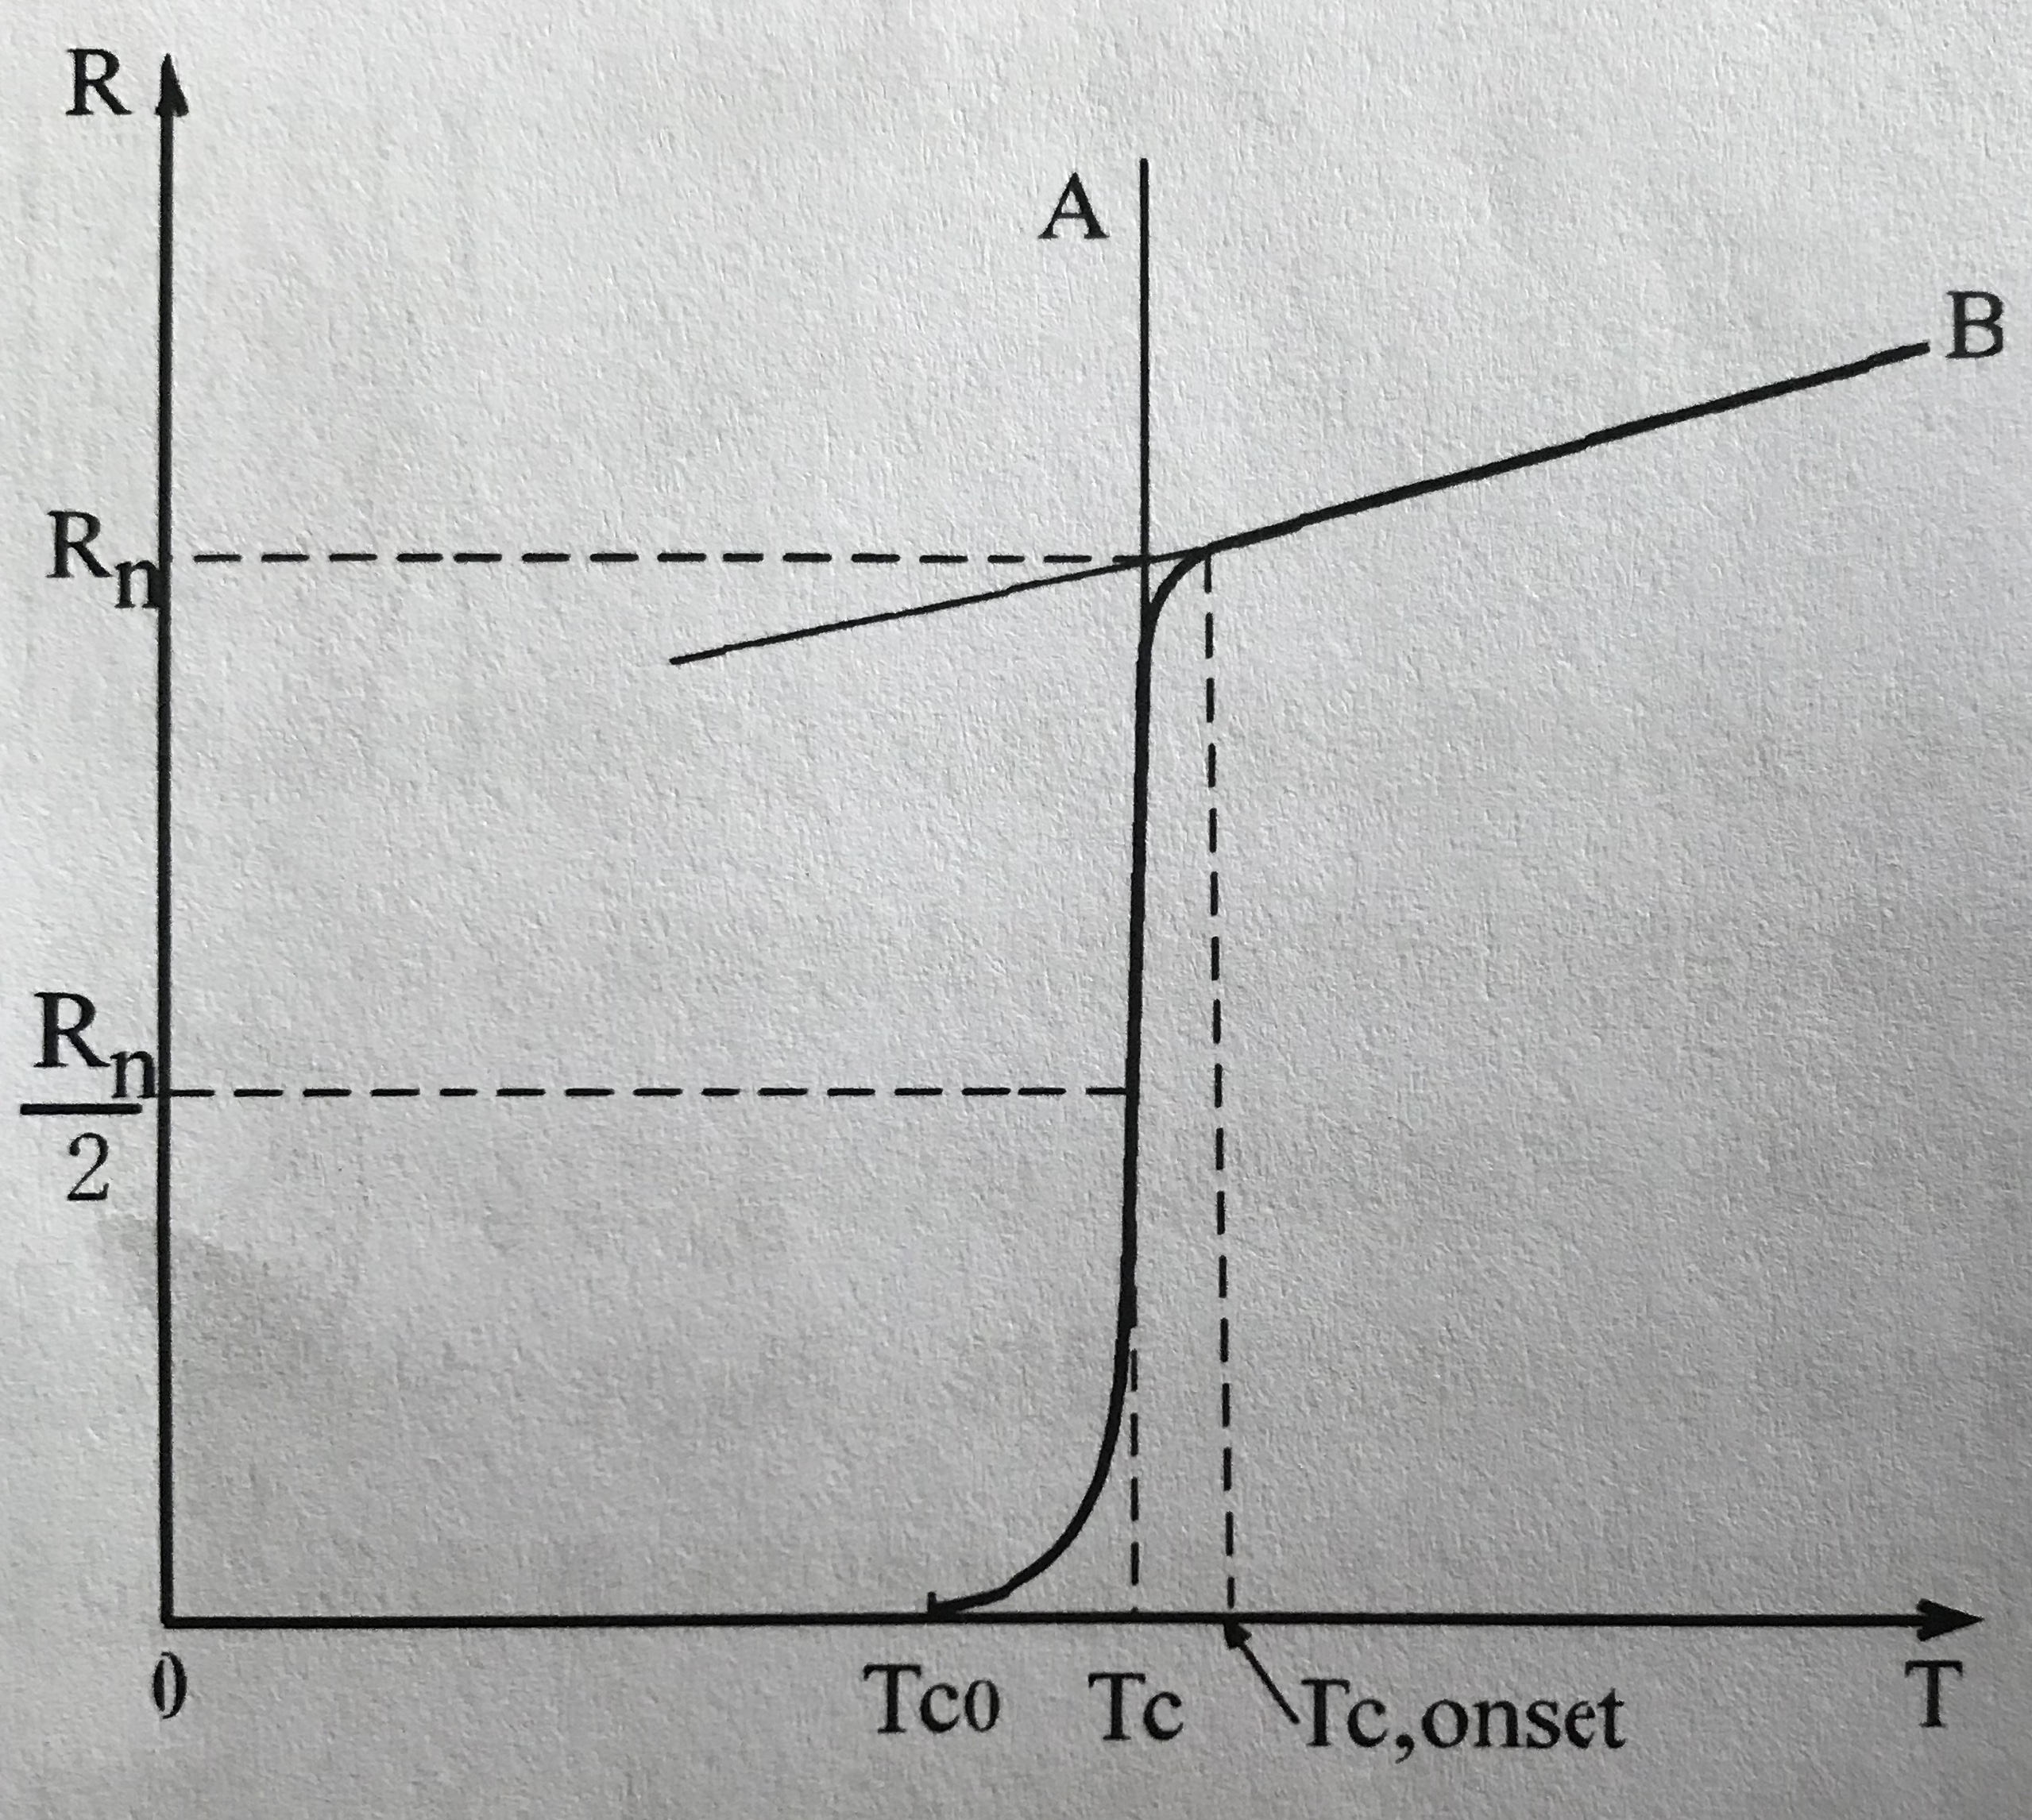
\includegraphics[width=4cm]{2.jpg}
\caption{\small{超导体的电阻转变曲线}}
\end{figure}
实验上,用电阻法测定临界温度时,如图1有:
\newline\textbf{转变温度$T_{c,onset}$}:降温过程中电阻温度曲线开始从直线偏离处的温度.
\newline\textbf{临界温度$T_c$(中点温度$T_{cm}$)}:待测样品电阻从起始转变处下降到一半时对应的温度。
\newline\textbf{转变宽度$\Delta T_{c}$}:电阻变化10%到90%所对应的温度间隔。
\newline\textbf{完全转变温度$T_{c0}$}:电阻刚刚完全降到零时的温度称为完全转变温度即零电阻温度。
\newline$\Delta T_{c}$的大小反映了材料品质的好坏,均匀单相的样品$\Delta T_{c}$较窄,反之较宽。
\subsubsection{迈纳斯效应}
超导体冷却到超导态后不存在内部磁场,不论是否处于磁场中,这个效应称之为迈斯纳效应。

\subsubsection{临界磁场$H_{c}$}
把一个磁场加到超导体上后,一定数量的磁场能量用来建立屏蔽电流的磁场以抵消超导体的内部磁场。当磁场达到某一定值时,它在能量上更有利于使样品返回正常态,允许磁场穿透,即破坏了超导电性。若超导体存在杂质和应力等,在超导体不同处有不同的$H_{c}$,因此转变将在一个很宽的范围内完成,$\rho=\rho_{0} / 2$相应的磁场叫临界磁场。

存在两类可区分的磁行为:
\newline\textbf{第\uppercase\expandafter{\romannumeral1}类超导体}:在$T_c$以下,临界磁场$H_{\mathrm{c}}(\mathrm{T})$随温度下降而增加,由实验拟合给出
\begin{equation}
H_{c}(T)=H_{c}(0)\left[1-\left(T / T_{c}\right)^{2}\right]
\end{equation}
\noindent\textbf{第\uppercase\expandafter{\romannumeral2}类超导体}:在超导态和正常态之间存在过渡的中间态,因此第\uppercase\expandafter{\romannumeral2}类超导体
存在两个临界磁场$H_{c1}$和$H_{c2}$。$H<H_{c1}$时,具有和第\uppercase\expandafter{\romannumeral1}类超导体相同的迈斯纳态的磁矩,$H_{c1}$称为下临界磁场;$H>H_{c1}$后,磁场将进入到超导体中,但这时体系仍有无阻的能力,随着磁场进入到超导体中增加超导态的比例减少,故磁化曲线缓慢减小直至为零,超导体完全恢复到正常态,此时的$H_{c2}$称为上临界磁场;$H_{c1}<H<H_{c2}$区域的状态为混合态。
\begin{figure}[H]
\centering
  \subfigure[第\uppercase\expandafter{\romannumeral1}类超导体]{ 
    \label{fig:subfig:a} %% label for first subfigure 
    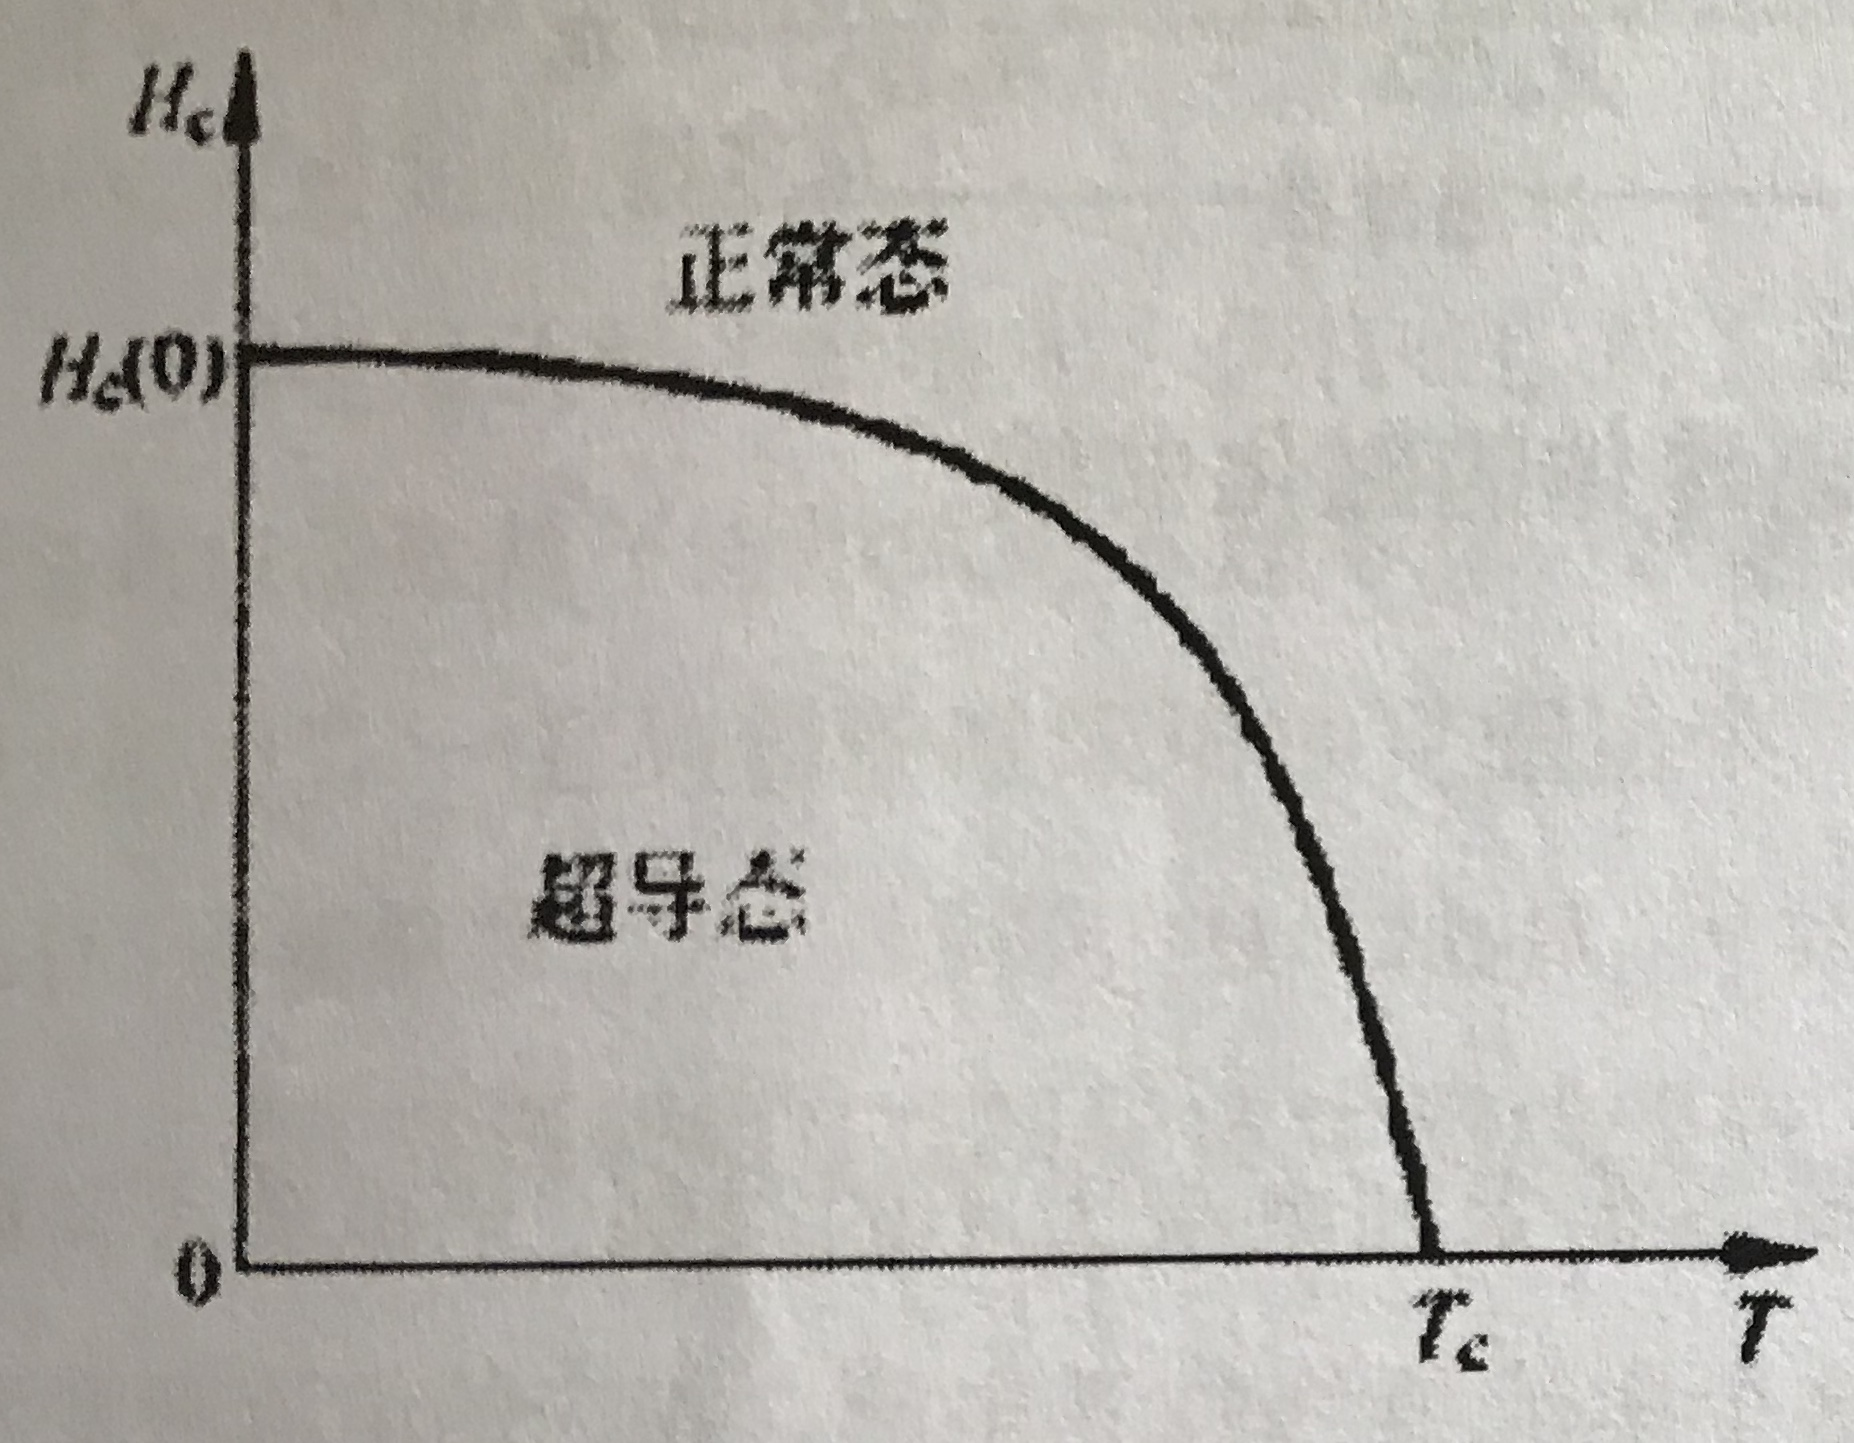
\includegraphics[width=3.5cm]{4.jpg}} 
  \subfigure[第\uppercase\expandafter{\romannumeral2}类超导体]{ 
    \label{fig:subfig:b} %% label for second subfigure 
    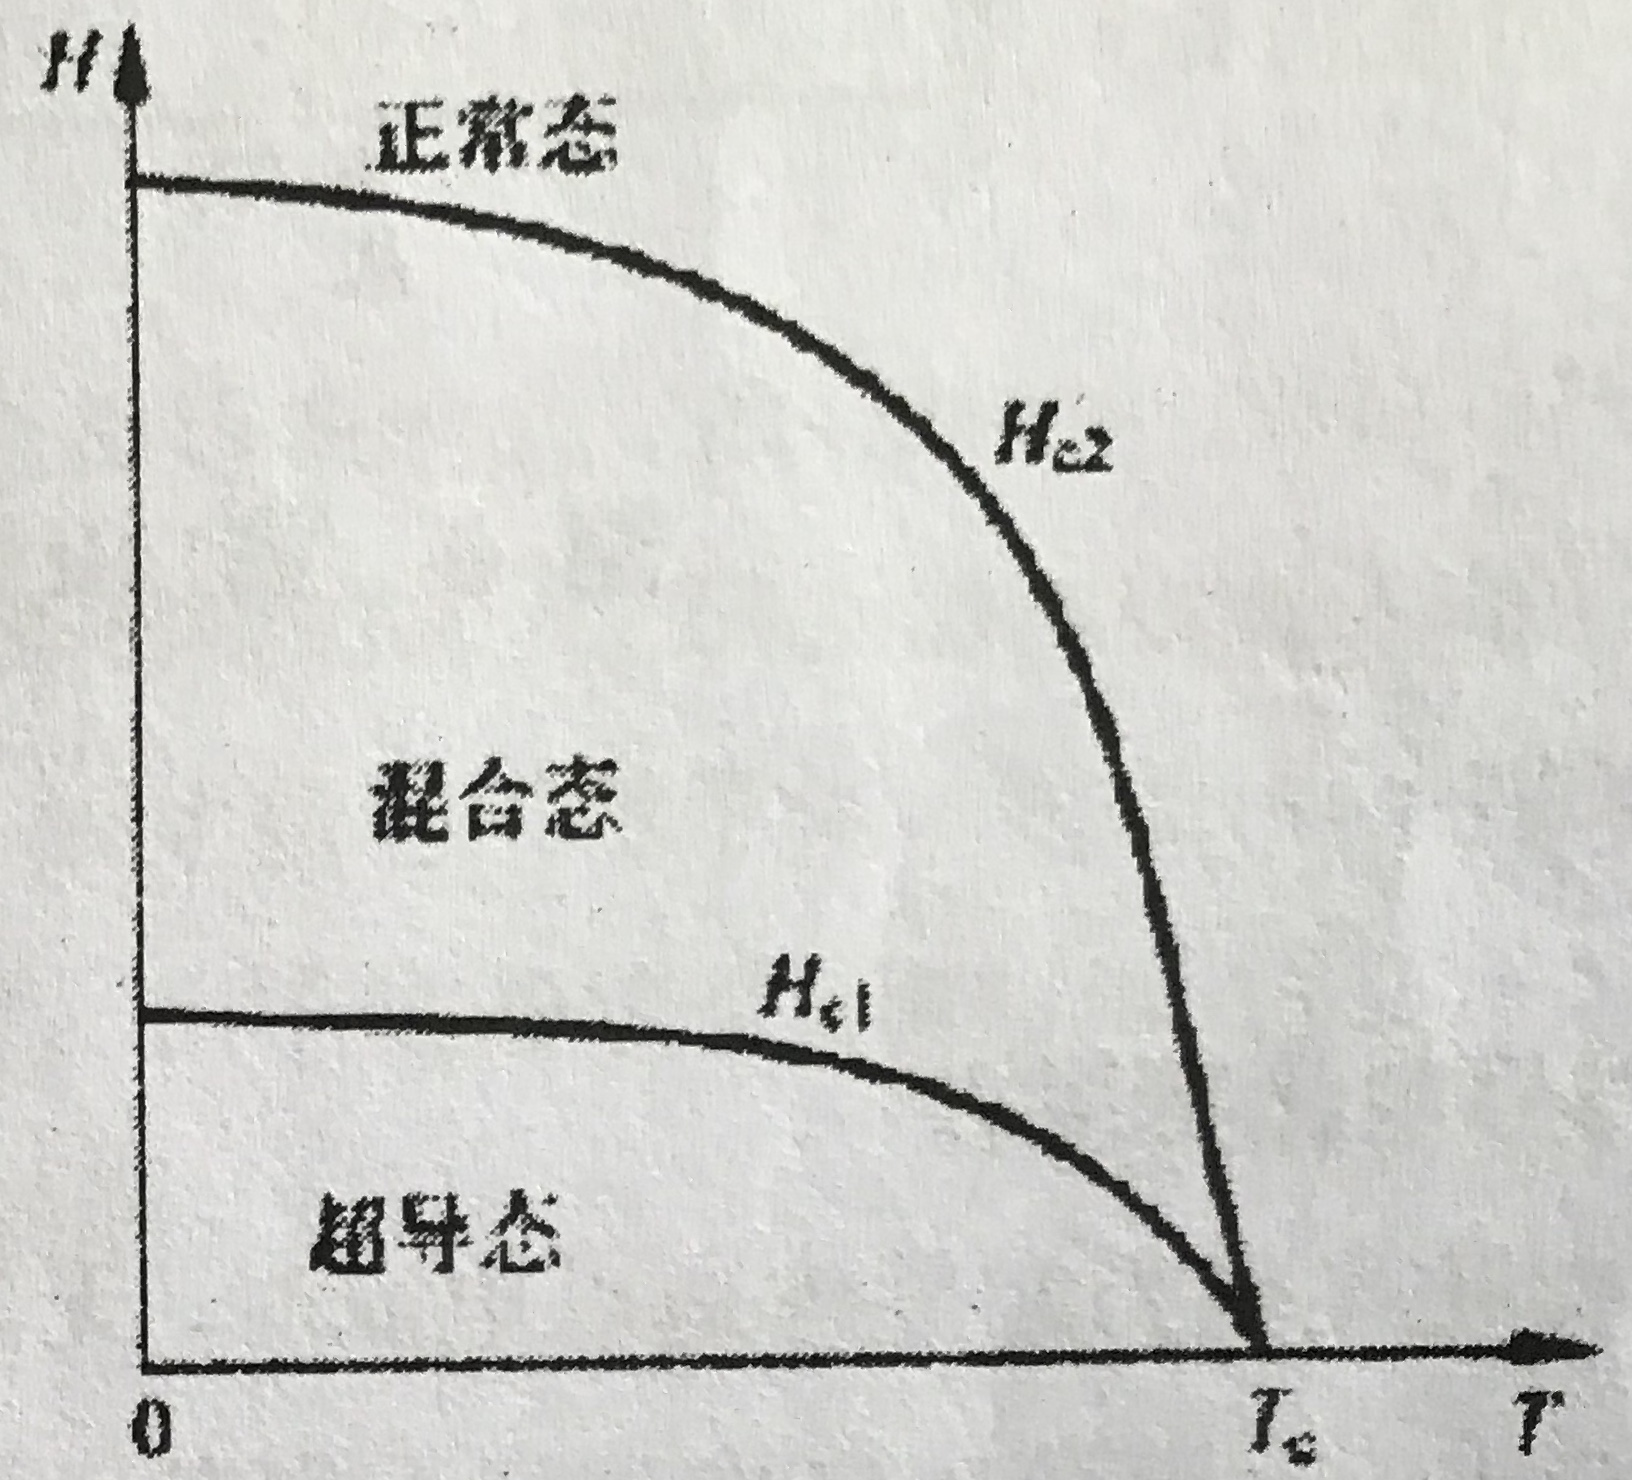
\includegraphics[width=3.5cm]{5.jpg}} 
  \caption{临界磁场随温度变化} 
  \label{fig:subfig} %% label for entire figure 
\end{figure}
\begin{figure}[H]
\centering
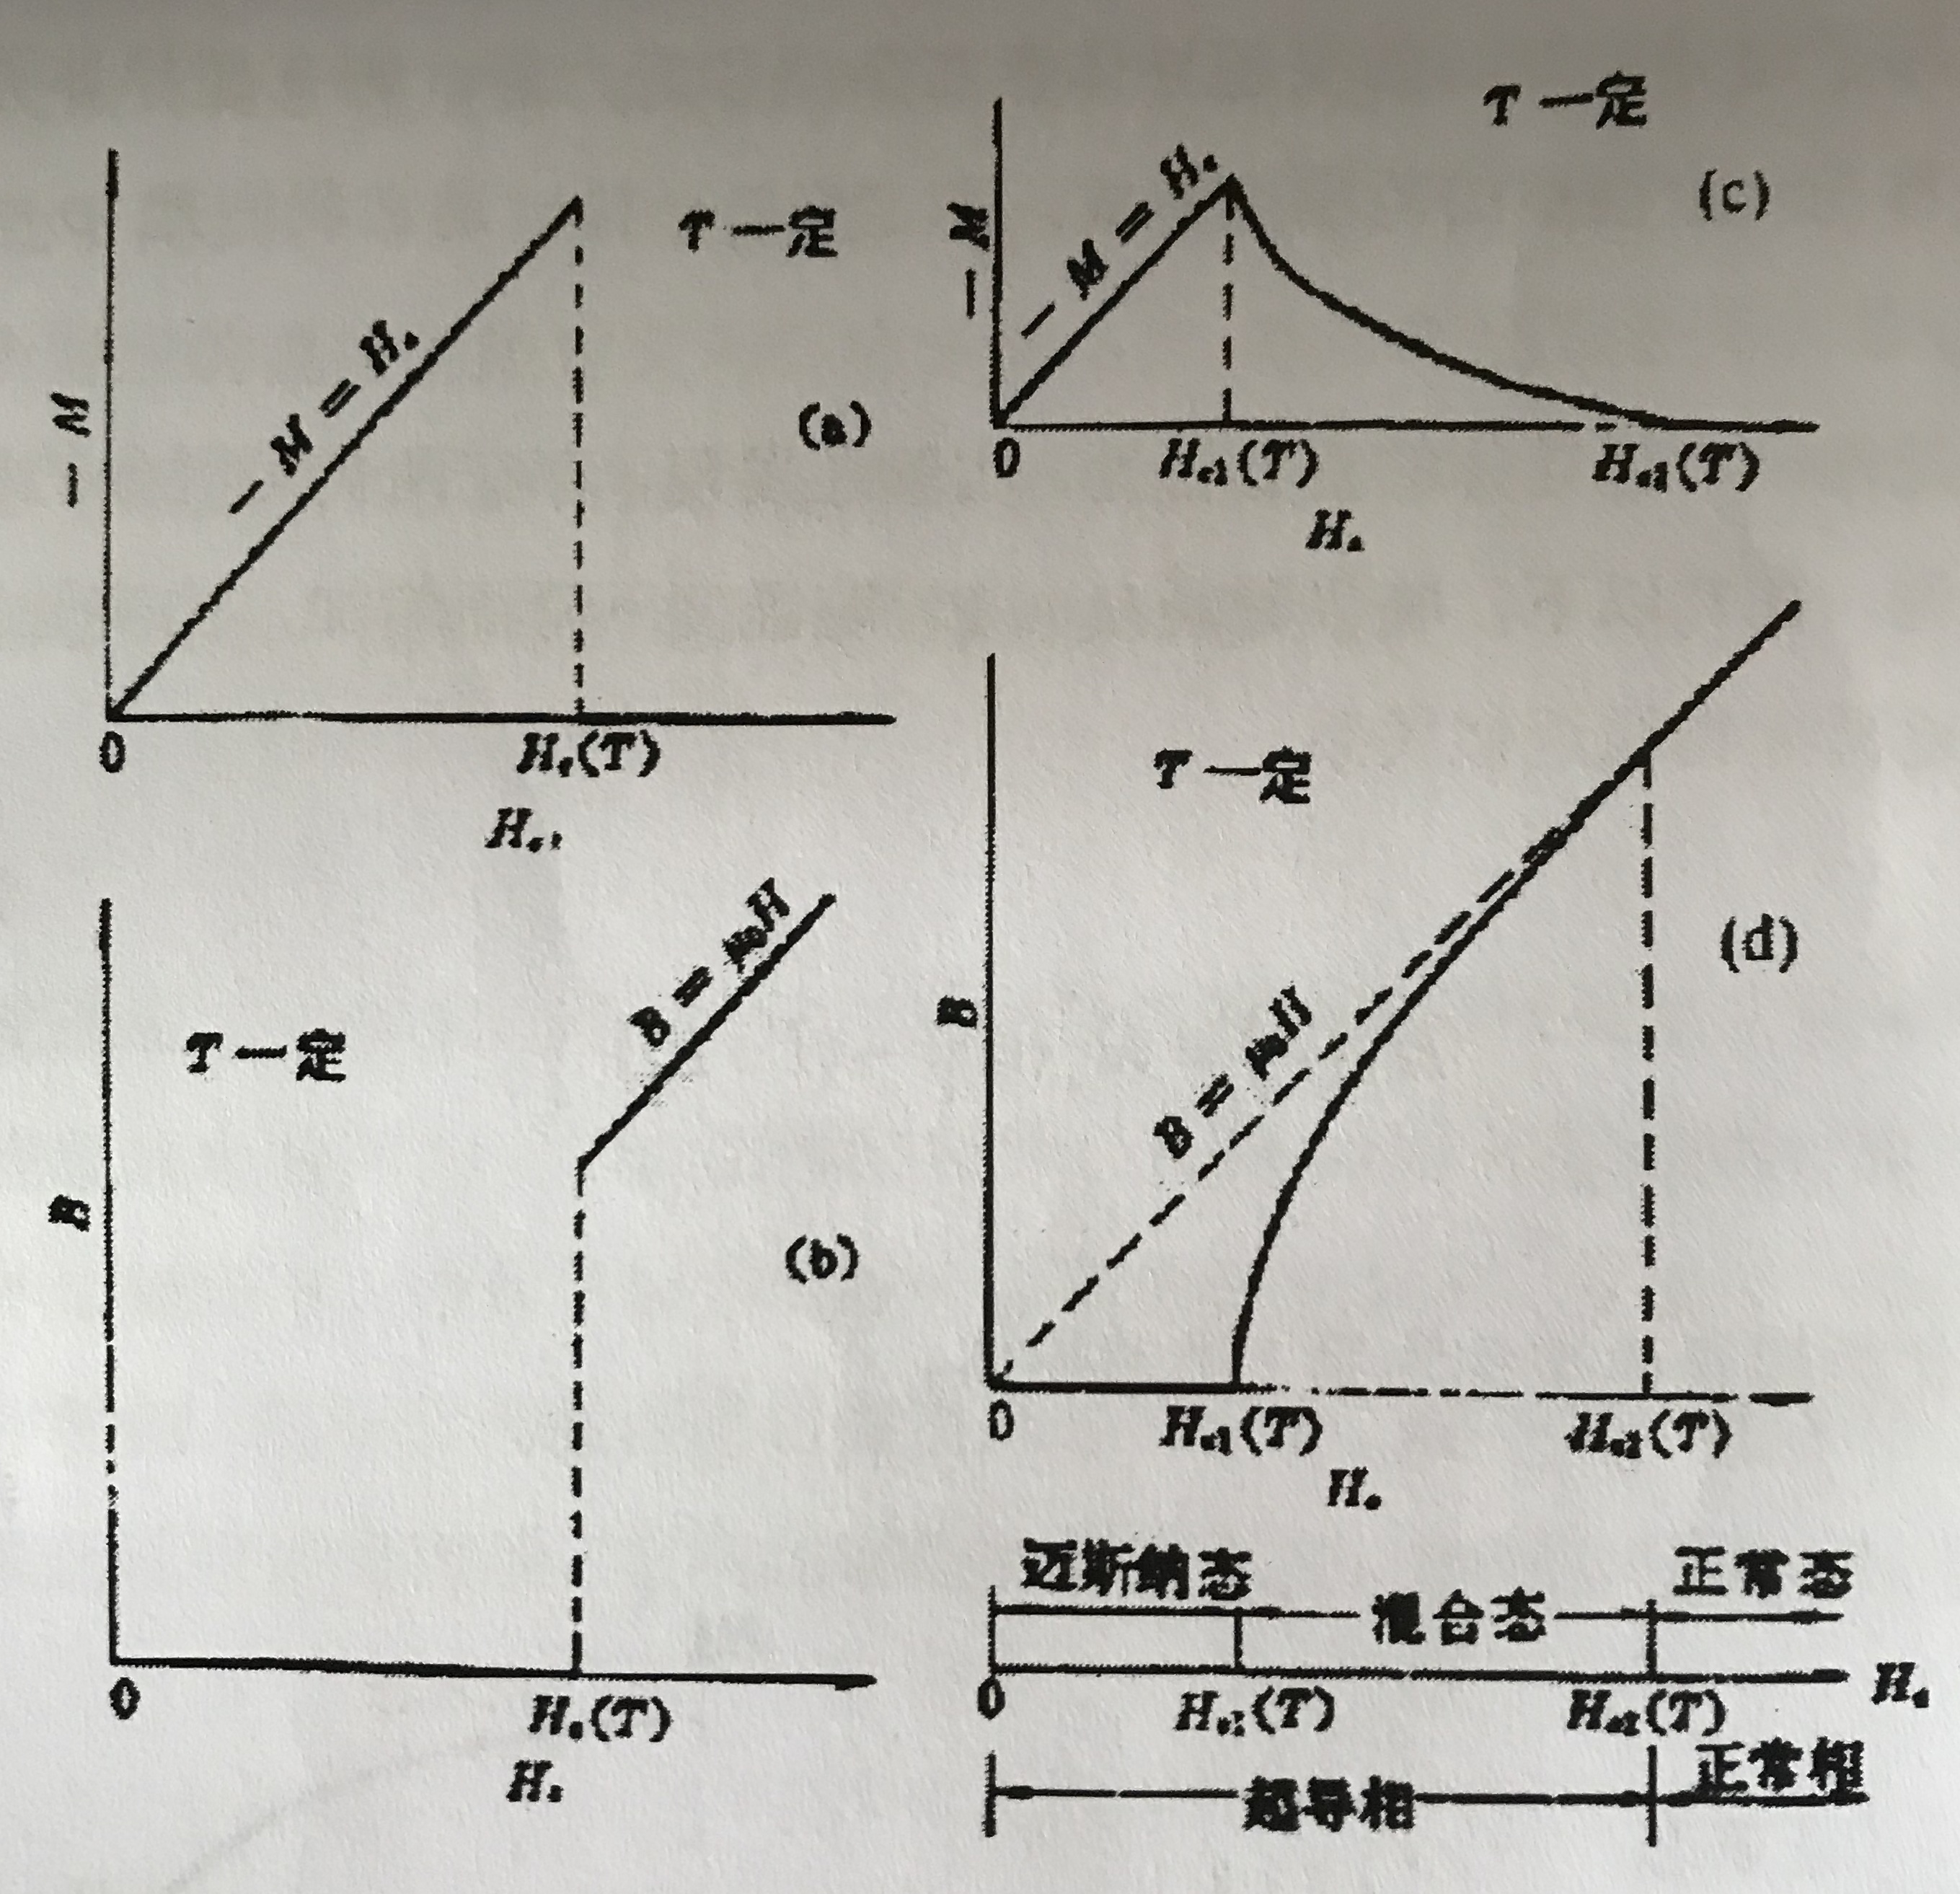
\includegraphics[width=8cm]{6.jpg}
\caption{\small{磁化曲线}}
\end{figure}

\subsubsection{临界电流密度$J_{c}$}
当超导体通以电流,无阻的超流态受到电流大小的限制,当电流达到某临界值后,超导体将恢复到正常态,称该电流值为临界电流,相应的电流密度为临界电流密度。对大多数金属超导体正常态的恢复是突变的;而对超导合金、化合物及高温超导体,电阻随增加渐变到正常电阻。临界电流与临界磁场强度$H_{c}$相关,外加磁场越强,临界电流就越小。临界磁场强度$H_{c}$依赖于温度,随温度升高而减小,并在转变温度$T_{c}$时降为零。临界电流密度$J_{c}$在较高温度下减小。
临界温度$T_{c}$,临界电流密度$J_{c}$和临界磁场$H_{c}$是超导体的3个临界参数,这3个参数与物质的内部微观结构有关。要使超导体处于超导态,必须将其置于这3个临界值以下,只要其中任何一个条件被破坏,超导态都会被破坏。
\subsubsection{实用超导体——非理想的第\uppercase\expandafter{\romannumeral2}类超导体}
\noindent\textbf{(1)磁通俘获和不可逆磁化}

对实用超导体——非理想的第\uppercase\expandafter{\romannumeral2}类超导体,当$H>H_{c1}$,磁通线可进入超导体中,且外磁场移去后,超导体中仍存在磁通俘获。

当外磁场从零开始增加,$H<H_{c1}$时,超导体处在迈斯纳态,故$-M=H$;$H>H_{c1}$时,磁场将以磁通量子的形式进入超导体,缺陷阻碍了磁通线的进入,因此磁通线进入超导体受到“阻力”,一直到磁场继续增加克服这个“阻力”后才能进入超导体,故在$-M-H$曲线上,$H>H_{c1}$还要继续上升;同样,H从$H>H_{c1}$开始下降时,磁通线受到阻力,不易排出,形成了磁通俘获。
\begin{figure}[H]
\centering
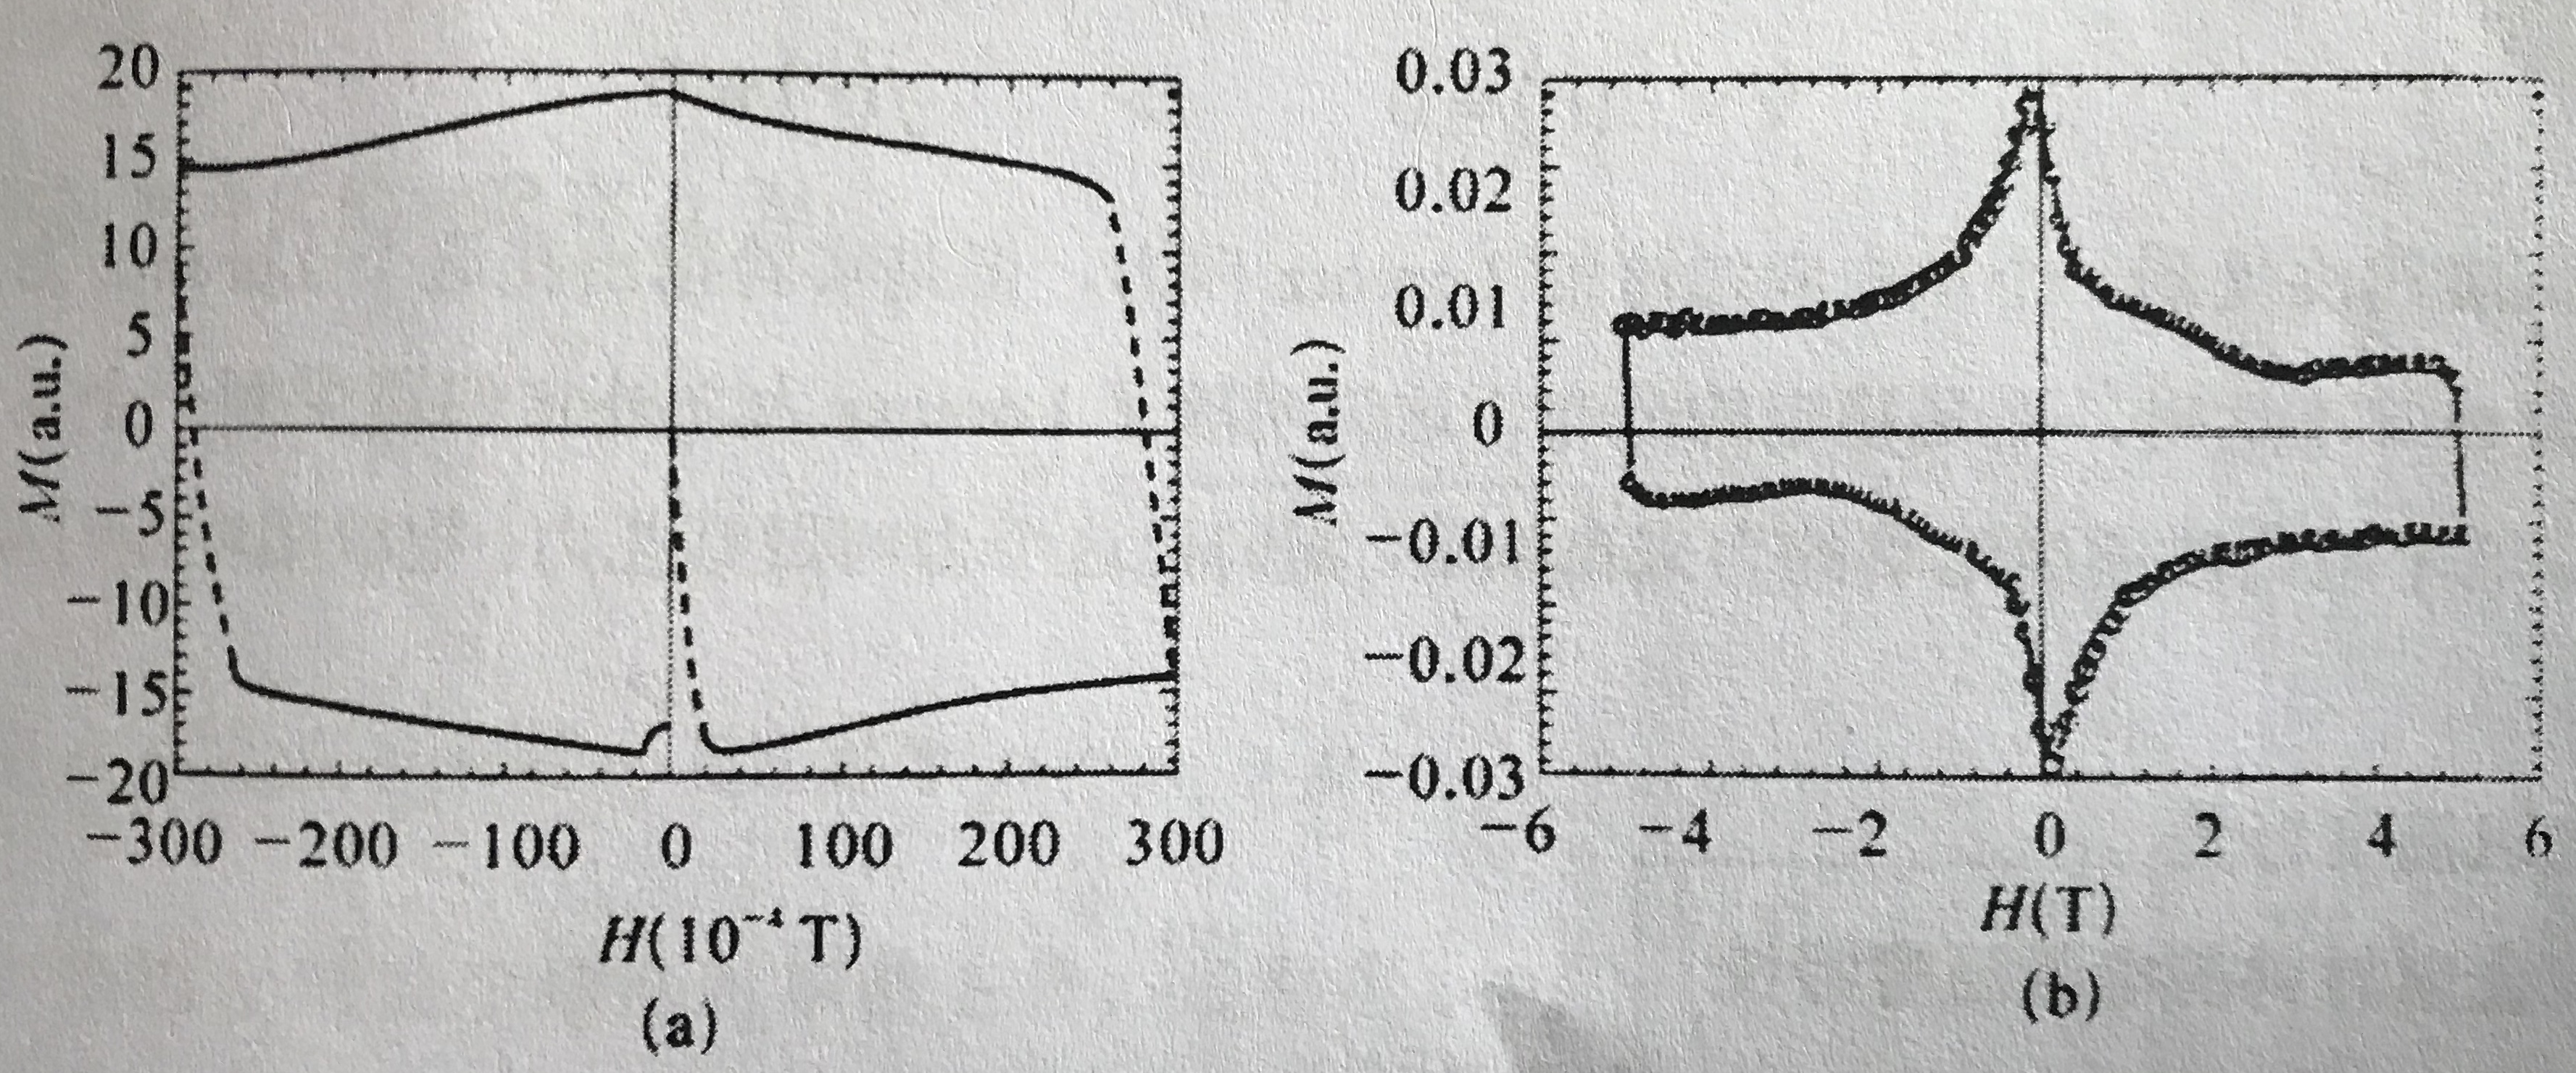
\includegraphics[width=8cm]{8.jpg}
\caption{\small{YBCO的磁化曲线,a.弱场,b.强场}}
\end{figure}

\noindent\textbf{(2)钉扎力和钉扎中心}

理想第\uppercase\expandafter{\romannumeral2}类超导体中的涡旋线分布是均匀的三角形点阵,因为涡旋线是均匀分布的,超导体中的磁感应强度$B(r)$不依赖于$r$,故$\mu_{0}\vec{j}(\vec{r})=\nabla \times \vec{B}(\vec{r})=0$。

非理想第\uppercase\expandafter{\romannumeral2}类超导体中涡旋线是不均匀分布的,超导体中的磁感应强度$B(r)$与空间位置有关,故$\vec{B}(\vec{r})\neq0$,$\vec{j}(\vec{r})\neq0$。因此涡旋线将受到一个从内向边缘的Lorentz斥力。但是实验指出在这个Lorentz力的作用下涡旋线由于钉扎力阻碍而稳定地分布,钉扎力来自缺陷,把缺陷称为钉扎中心。

\subsection{电阻温度特性}
\subsubsection{纯金属材料的电阻温度特性}
金属中总电阻率表示为
\begin{equation}
\rho=\rho_{L}(T)+\rho_{r}
\end{equation}
$\rho_{L}(T)$为晶格热振动对电子散射引起的电阻率,与温度有关,相关性由晶格散射决定。金属能带理论计算得:在高温区,$T>\Theta_{D} / 2$时,$\rho_{L}(T)\propto T$;在低温区,$T<\Theta_{D} /10$时,$\rho_{L}(T)\propto T^5$。其中$\Theta_{D}$为德拜温度。

$\rho_{r}$为杂质和缺陷对电子的散射所引起的电阻率,与杂质和缺陷的密度成正比,称为剩余电阻率。也就是说,杂质和缺陷可以改变金属电阻率的数值,但不改变电阻率的温度系数。

在液氮正常沸点到室温温度范围内,铂电阻与温度具有良好的线性关系。

\subsubsection{半导体材料的电阻温度特性}
本征半导体的电阻率为
\begin{equation}
\rho_{i}=\frac{1}{n_{i} e\left(\mu_{e}+\mu_{p}\right)}
\end{equation}
$\rho_{i}$由载流子浓度$n_{i}$及迁移率$\mu = \mu_{e}+\mu_{p}$决定,但因$n_{i}$随温度增高而指数上升,迁移率$\mu$随温度增高而下降较慢,故本征半导体的电阻率$\rho_{i}$随温度上升而单调下降$d \rho_{i} / d T<0$。

半导体在一定温度范围内具有负的电阻温度系数,根据半导体低温区电阻温度关系,用半导体材料做成的温度计,可以弥补金属电阻温度计在低温区电阻值和灵敏度降低的缺陷。常用的半导体温度计有锗电阻温度计、硅电阻温度计、碳电阻温度计和热敏电阻温度计。

\section{实验仪器}
(1)低温温度的获得和控制主要包括低温恒温器和不锈钢杜瓦容器;(2)电测量部分主要包括BW2型高温超导材料特性测试装置和PZ158型直流数字电压表;(3)高温超导体的磁悬浮演示装置

\section{实验内容}
\subsection{检查电路的连接与开机}
检查如下的电路连接:19芯插头两端分别接在低温恒温器拉杆顶端和电源盒后侧面的插座上,电源机盒面板上虚线所示的待连接线,PZ158型直流电压表与面板上的“外接PZ158”接线柱连接。

按下PZ158型数字电压表开关,待自检校准后按下200mV档按键。

打开电源盒总开关,依次按下铂电阻温度计、硅二极管温度计和超导样品的电源开关(不要打开加热部分的开关)。校准通过铂电阻温度计和硅二极管温度计标准电阻的电流,超导
样品电流一般设为5mA,此时,超导体样品的室温电压大约在50~100V之间。然后切换各换位旋钮的位置,记录各温度计在室温下的电流和电压数据。
\subsection{液氮的灌注}
液氮加注过程中,要十分小心注意防止液氮溅到裸露的皮肤上。另外,要注意防止变硬的输液器胶管被弄碎检查不锈钢杜瓦瓶,确保其中无残留的杂物,否则须清理干净

灌注液氮时,输液器胶管会冻硬,而弯曲状的胶管会使被压出的液氮喷流不畅,故应先整理好液氮罐到杜瓦瓶的距离,使胶管除插入杜瓦瓶约10cm外,在两罐间基本保持直线状。

将金属管插入液氮罐的同时将胶管插入杜瓦瓶,按紧橡胶塞。然后,关闭输液器上端的通气阀,此时由于罐内压强升高,液氮将通过输液管开始注入不锈钢杜瓦瓶中。当气压不够时,可平缓地压迫输液管上端的气球,使液氮继续被压出。液氮加注量可用直尺测量确定,以静止后的液面到瓶口距离30cm左右为宜。

液氮加注完毕,将输液器上端通气阀打开,慢慢将输液器取出,让剩余液氮回流干净,立于液氮罐旁,将液氮罐盖好。
\subsection{恒温器与液氮表面相对位置的控制}
保持恒温器与液氮表面的间距在几个毫米是在规定的时间内顺利完成实验的关键,必须在整个降温过程中格外细心。如使恒温器浸入液氮,则超导样品迅速达到液氮温度而成超导状态,这样就无法测出转变温度,致使实验失败。

1.用直尺精确测量液氮表面到杜瓦瓶口的距离,松开恒温器上杜瓦瓶盖板外侧的引线拉杆锁定螺母,调整盖板位置,使盖板内侧到恒温器下挡板的间距比液氮表面到杜瓦瓶瓶口
的距离略长2~3mm,不可超出5mm,以使恒温器放入杜瓦瓶后下挡板刚好浸入液氮。然后固定好拉杆锁定螺母。

2.将电源盒超导样品部分的测量转换开关旋至“液面计”处,再将恒温器缓缓地放入杜瓦瓶中。当恒温器的下挡板浸入液氮时,会因液氮沸腾而喷出冷气并伴随轻微的液体沸腾声,此时,盖板应基本到瓶口位置,将杜瓦瓶盖好。若此时盖板距瓶口距离大于1cm,要立即停止下插,并松开拉杆锁定螺母,下调盖板以确保避免恒温器直接浸入液氮。

待1分钟后,液面逐渐平静时稍许旋松拉杆锁定螺母,使恒温器缓缓下降,同时密切监视PZ158数字电压表,当其电压值减小到零时,立即拧紧固定螺母,此时液氮表面刚好处于液面计热电偶上结点的上方。

下调恒温器时,可将直尺立于杜瓦瓶盖板上,观察拉杆顶端方形引线座研直尺刻度下移量,每次移动约2mm,切莫过多。若发现电表变化过快,或其他不正常则要立即将恒温器稍稍上提。对液面计需要注意的是,恒温器下移后液面计电压的下降可能滞后十几秒到半分钟
,及由于液面的不稳定和液面计导线的不均匀,液面计会有$\pm(2 \sim 3) \mu V$的示数

3.由于液氮的消耗,液面会不断下降,因此,在整个测量过程中,要随时调节恒温器的位置以保持其与液氮表面的相对位置。一旦发现液面计电压不为零,就应将拉杆向下移动少许,使电压恢复到零。

4.多次实验后,样品与恒温器的接触可能因热胀冷缩而变差,此时应适当减少下挡板到液面的距离。
\subsection{超导转变曲线的测量}
由于铂电阻温度计性能稳定,且有较好的电阻温度关系,我们由铂电阻温度计测出温度,再测出相应温度下的其他3个参量:硅二极管温度计pn结的正向电压、温差热电偶的温差电动势和超导样品的电压。具体方法是将铂R-T对照表上的电阻值换成电压值,然后监视铂电阻温度计的电压,每达到一个指定的电压,即达到指定温度时,对其他3个参量进行测量。

1.恒温器刚放入液氮罐时温度降得较快,这时可连续进行测量和记录。在连续测量4~5点后,降温速度开始变慢,此时参照铂电阻R-T对照表,从当前温度开始,大约每隔表上给出的5个值进行1次测量。

2当恒温器的温度降到约130K时,接近超导转变温度,应加密测量点,此时对铂电阻R-T对照表上标出的每两个值进行1次测量。

3.当接近起始转变温度时,样品电压的下降变快。这时温度约93K,此后很快开始发生超导转变,在此过程中,要求约每隔30秒测量一次。

4.到达零电阻温度后,样品电压为零。此时为确保测量的准确,应将电流反向,记录样品的正、反向电压。若正、反电流下测得的电阻值均为零,表明样品已进入零电阻状态。此后继续每隔30秒测量3~5个点。

5.为完成低温温度计的标定,此后,继续每隔铂电阻R-T对照表上的两个值进行1次测量,直到液氮温度。

6.完成实验测量后,将恒温器缓缓取出并松开拉杆锁定螺母。

\subsection{高温超导体磁悬浮演示及磁悬浮力测量}
在场冷和零场冷条件下冷却超导盘片至超导态,进行观察,并使用仪器测量其磁悬浮力,得到超导体-磁体间距关系曲线。

\end{multicols}

\section{实验结果分析与讨论}
\subsection{超导样品电阻随温度的变化曲线}
恒定电流$I=5mA$
\begin{table}[H]
\tiny
\begin{tabular}{|l|l|l|l|l|l|l|l|l|l|l|l|l|l|l|l|}
\hline
温度/K          & 285.7  & 280.1  & 276.7  & 276.12 & 268.01 & 254.42 & 241.82 & 229.46 & 223.53 & 218.51 & 213.36 & 209.01 & 203.52 & 199.14 & 194.21  \\ \hline
样品电压/$mv$ & 0.084  & 0.081  & 0.081  & 0.078  & 0.078  & 0.076  & 0.075  & 0.075  & 0.074  & 0.074  & 0.074  & 0.073  & 0.072  & 0.071  & 0.071   \\ \hline
温度/K          & 187.37 & 181.18 & 173.88 & 167.01 & 160.88 & 155.51 & 150.65 & 144.01 & 137.15 & 129.92 & 124.76 & 118.05 & 112.19 & 105.98 & 100.860 \\ \hline
样品电阻/$mV$ & 0.071  & 0.07   & 0.069  & 0.067  & 0.065  & 0.064  & 0.063  & 0.063  & 0.062  & 0.061  & 0.06   & 0.057  & 0.056  & 0.055  & 0.053   \\ \hline
温度/K          & 94.585 & 93.178 & 93.154 & 93.303 & 93.061 & 92.967 & 92.944 & 92.850 & 92.780 & 92.663 & 92.522 & 92.335 & 92.194 & 92.124 &         \\ \hline
样品电阻/$mV$ & 0.048  & 0.039  & 0.038  & 0.036  & 0.034  & 0.032  & 0.031  & 0.029  & 0.027  & 0.024  & 0.021  & 0.018  & 0.015  & 0.013  &         \\ \hline
温度/K          & 91.913 & 91.773 & 91.609 & 91.468 & 91.328 & 91.164 & 90.976 & 90.623 & 90.389 & 90.084 & 83.047 & 81.476 & 78.011 & 77.730 &         \\ \hline
样品电阻/$mV$ & 0.01   & 0.008  & 0.006  & 0.004  & 0.003  & 0.001  & 0      & -0.001 & -0.003 & -0.002 & -0.002 & -0.003 & -0.003 & -0.003 &         \\ \hline
\end{tabular}
\end{table}

\begin{figure}[H]
\centering
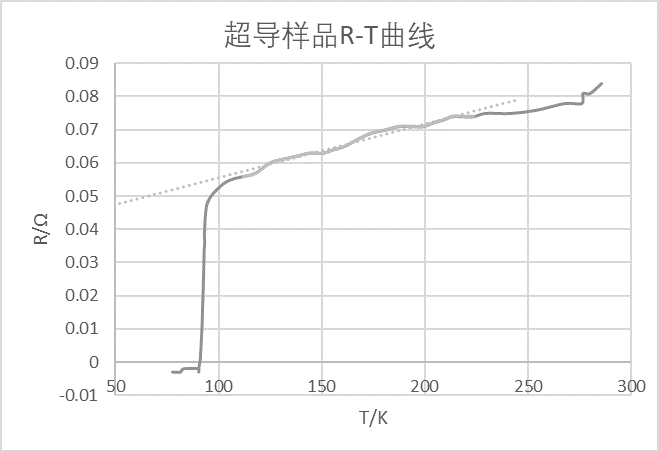
\includegraphics[width=10cm]{pic1.png}
\end{figure}

起始转变温度$T_{c,onset}$=105.98K;
零电阻温度$T_{c0}$=90.39K;
超导转变温度$T_{cm}$=92.78K。由图可见,当温度低于起始转变温度时,超导体的电阻突然跌落到零。

\subsection{金属的电阻率随温度的变化规律}
\begin{table}[H]
\tiny
\centering
\begin{tabular}{|l|l|l|l|l|l|l|l|l|l|l|l|l|l|l|l|}
\hline
温度/K         & 285.7  & 280.1  & 276.7  & 276.12 & 268.01 & 254.42 & 241.82 & 229.46 & 223.53 & 218.51 & 213.36 & 209.01 & 203.52 & 199.14 & 194.21 \\ \hline
Pt电阻/$\Omega$ & 105.06 & 102.8  & 101.4  & 100.8  & 98.14  & 92.72  & 87.8   & 82.8   & 80.5   & 78.5   & 76.4   & 74.7   & 72.5   & 70.2   & 68.8   \\ \hline
温度/K         & 187.37 & 181.18 & 173.88 & 167.01 & 160.88 & 155.51 & 150.65 & 144.01 & 137.15 & 129.92 & 124.76 & 118.05 & 112.19 & 105.98 & 100.86 \\ \hline
Pt电阻/$\Omega$ & 66     & 63.5   & 60.57  & 57.75  & 55.25  & 53.1   & 51.1   & 48.3   & 45.5   & 42.5   & 40.35  & 37.58  & 35.1   & 32.42  & 30.28  \\ \hline
温度/K         & 94.585 & 93.178 & 93.154 & 93.303 & 93.061 & 92.967 & 92.944 & 92.850 & 92.780 & 92.663 & 92.522 & 92.335 & 92.194 & 92.124 & 91.913 \\ \hline
Pt电阻/$\Omega$ & 27.62  & 27.02  & 27.01  & 27     & 26.97  & 26.93  & 26.92  & 26.88  & 26.85  & 26.8   & 26.74  & 26.66  & 26.6   & 26.57  & 26.48  \\ \hline
温度/K         & 91.773 & 91.609 & 91.468 & 91.328 & 91.164 & 90.976 & 90.623 & 90.389 & 90.084 & 83.047 & 81.476 & 78.011 & 77.730 &        &        \\ \hline
Pt电阻/$\Omega$ & 26.42  & 26.35  & 26.29  & 26.23  & 26.16  & 26.08  & 25.93  & 25.83  & 25.7   & 22.88  & 22.02  & 20.54  & 20.42  &        &        \\ \hline
\end{tabular}
\end{table}
\begin{figure}[H]
\centering
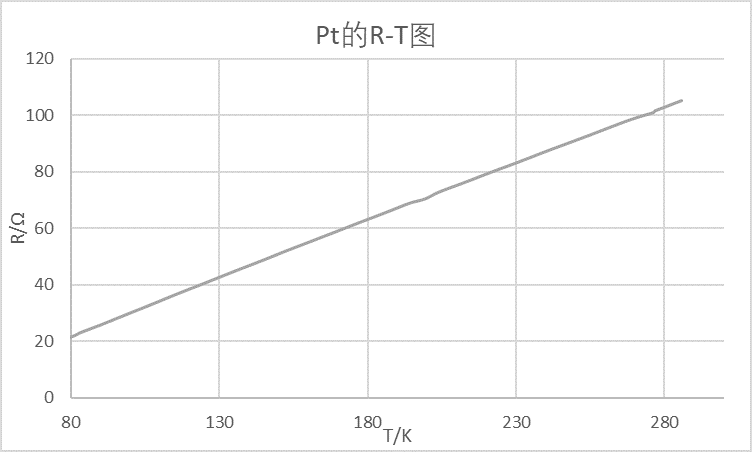
\includegraphics[width=10cm]{pic2.png}
\end{figure}
由图可见,在液氮正常沸点到室温温度范围内,铂电阻与温度具有良好的线性关系,$R(T)\propto T$。

\subsection{半导体的电阻率随温度的变化规律}
恒定电流$100\mu A$
\begin{table}[H]
\tiny
\centering
\begin{tabular}{|l|l|l|l|l|l|l|l|l|l|l|l|}
\hline
温度/K            & 285.7  & 280.1  & 276.7  & 276.12 & 268.01 & 254.42 & 241.82 & 229.46 & 223.53 & 218.51 & 213.36 \\ \hline
硅二极管电压/$V$ & 0.5313 & 0.5517 & 0.5617 & 0.565  & 0.5844 & 0.6126 & 0.642  & 0.6712 & 0.6851 & 0.6967 & 0.7089 \\ \hline
温度/K            & 209.01 & 203.52 & 199.14 & 194.21 & 187.37 & 181.18 & 173.88 & 167.01 & 160.88 & 155.51 & 150.65 \\ \hline
硅二极管电压/$V$ & 0.7188 & 0.73   & 0.745  & 0.7528 & 0.7689 & 0.7831 & 0.8    & 0.8163 & 0.8305 & 0.8424 & 0.85   \\ \hline
温度/K            & 144.01 & 137.15 & 129.92 & 124.76 & 118.05 & 112.19 & 105.98 & 100.86 & 94.585 & 93.178 &        \\ \hline
硅二极管电压/$V$ & 0.86   & 0.884  & 0.9    & 0.91   & 0.9275 & 0.941  & 0.9553 & 0.9663 & 0.9802 & 0.9834 &        \\ \hline
\end{tabular}
\end{table}

\begin{figure}[H]
\centering
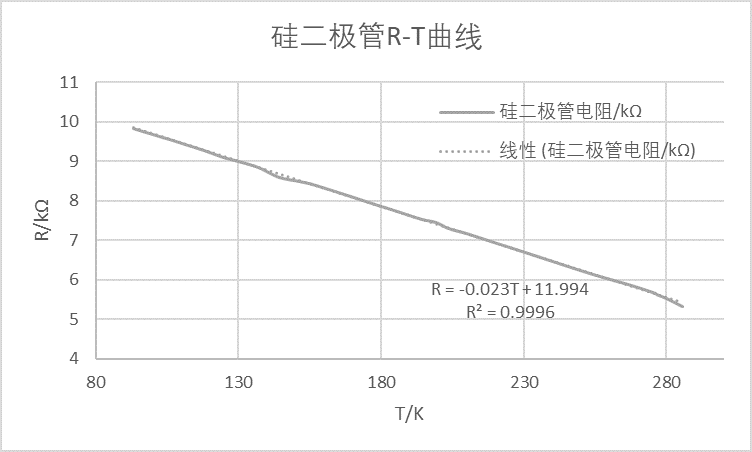
\includegraphics[width=10cm]{pic3.png}
\end{figure} 
由图可见,硅二极管电阻随温度下降而单调下降,是本征半导体。由趋势线可见,硅二极管随温度的变化趋于一阶线性递减。

\subsection{温差电偶随温度变化规律}
恒定电流$I=5mA$
\begin{table}[H]
\centering
\tiny
\begin{tabular}{|l|l|l|l|l|l|l|l|l|l|l|}
\hline
温度/K    & 285.7  & 280.1  & 276.7  & 276.12 & 268.01 & 254.42 & 241.82 & 229.46 & 223.53 & 218.51      \\\hline
温差电偶/mV & 4.233  & 5.428  & 5.246  & 5.203  & 4.861  & 4.43   & 3.947  & 3.84   & 3.664  & 3.506       \\\hline
温度/K    & 213.36 & 209.01 & 203.52 & 199.14 & 194.21 & 187.37 & 181.18 & 173.88 & 167.01 & 155.51      \\\hline
温差电偶/mV & 3.342  & 3.213  & 3.094  & 2.661  & 2.563  & 2.37   & 2.175  & 2.006  & 1.823  & 1.662       \\\hline
温度/K    & 150.65 & 144.01 & 137.15 & 129.92 & 124.76 & 118.05 & 112.19 & 105.98 & 100.86 & 94.58 \\\hline
温差电偶/mV & 1.533  & 1.418  & 1.258  & 1.101  & 0.948  & 0.837  & 0.696  & 0.578  & 0.467  & 0.373   \\ \hline   
\end{tabular}
\end{table}
\begin{figure}[H]
\centering
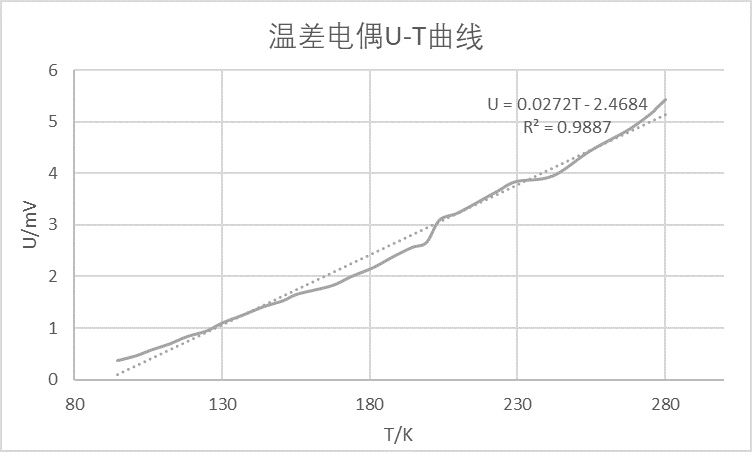
\includegraphics[width=10cm]{pic4.png}
\end{figure}
由图可见,温差热电偶电压随温度上升而上升。由趋势线可见,温差热电偶电压随温度的变化趋于一阶线性递增。

\subsection{高温超导体磁悬浮演示及磁悬浮力测量}
\begin{figure}[H]
\centering
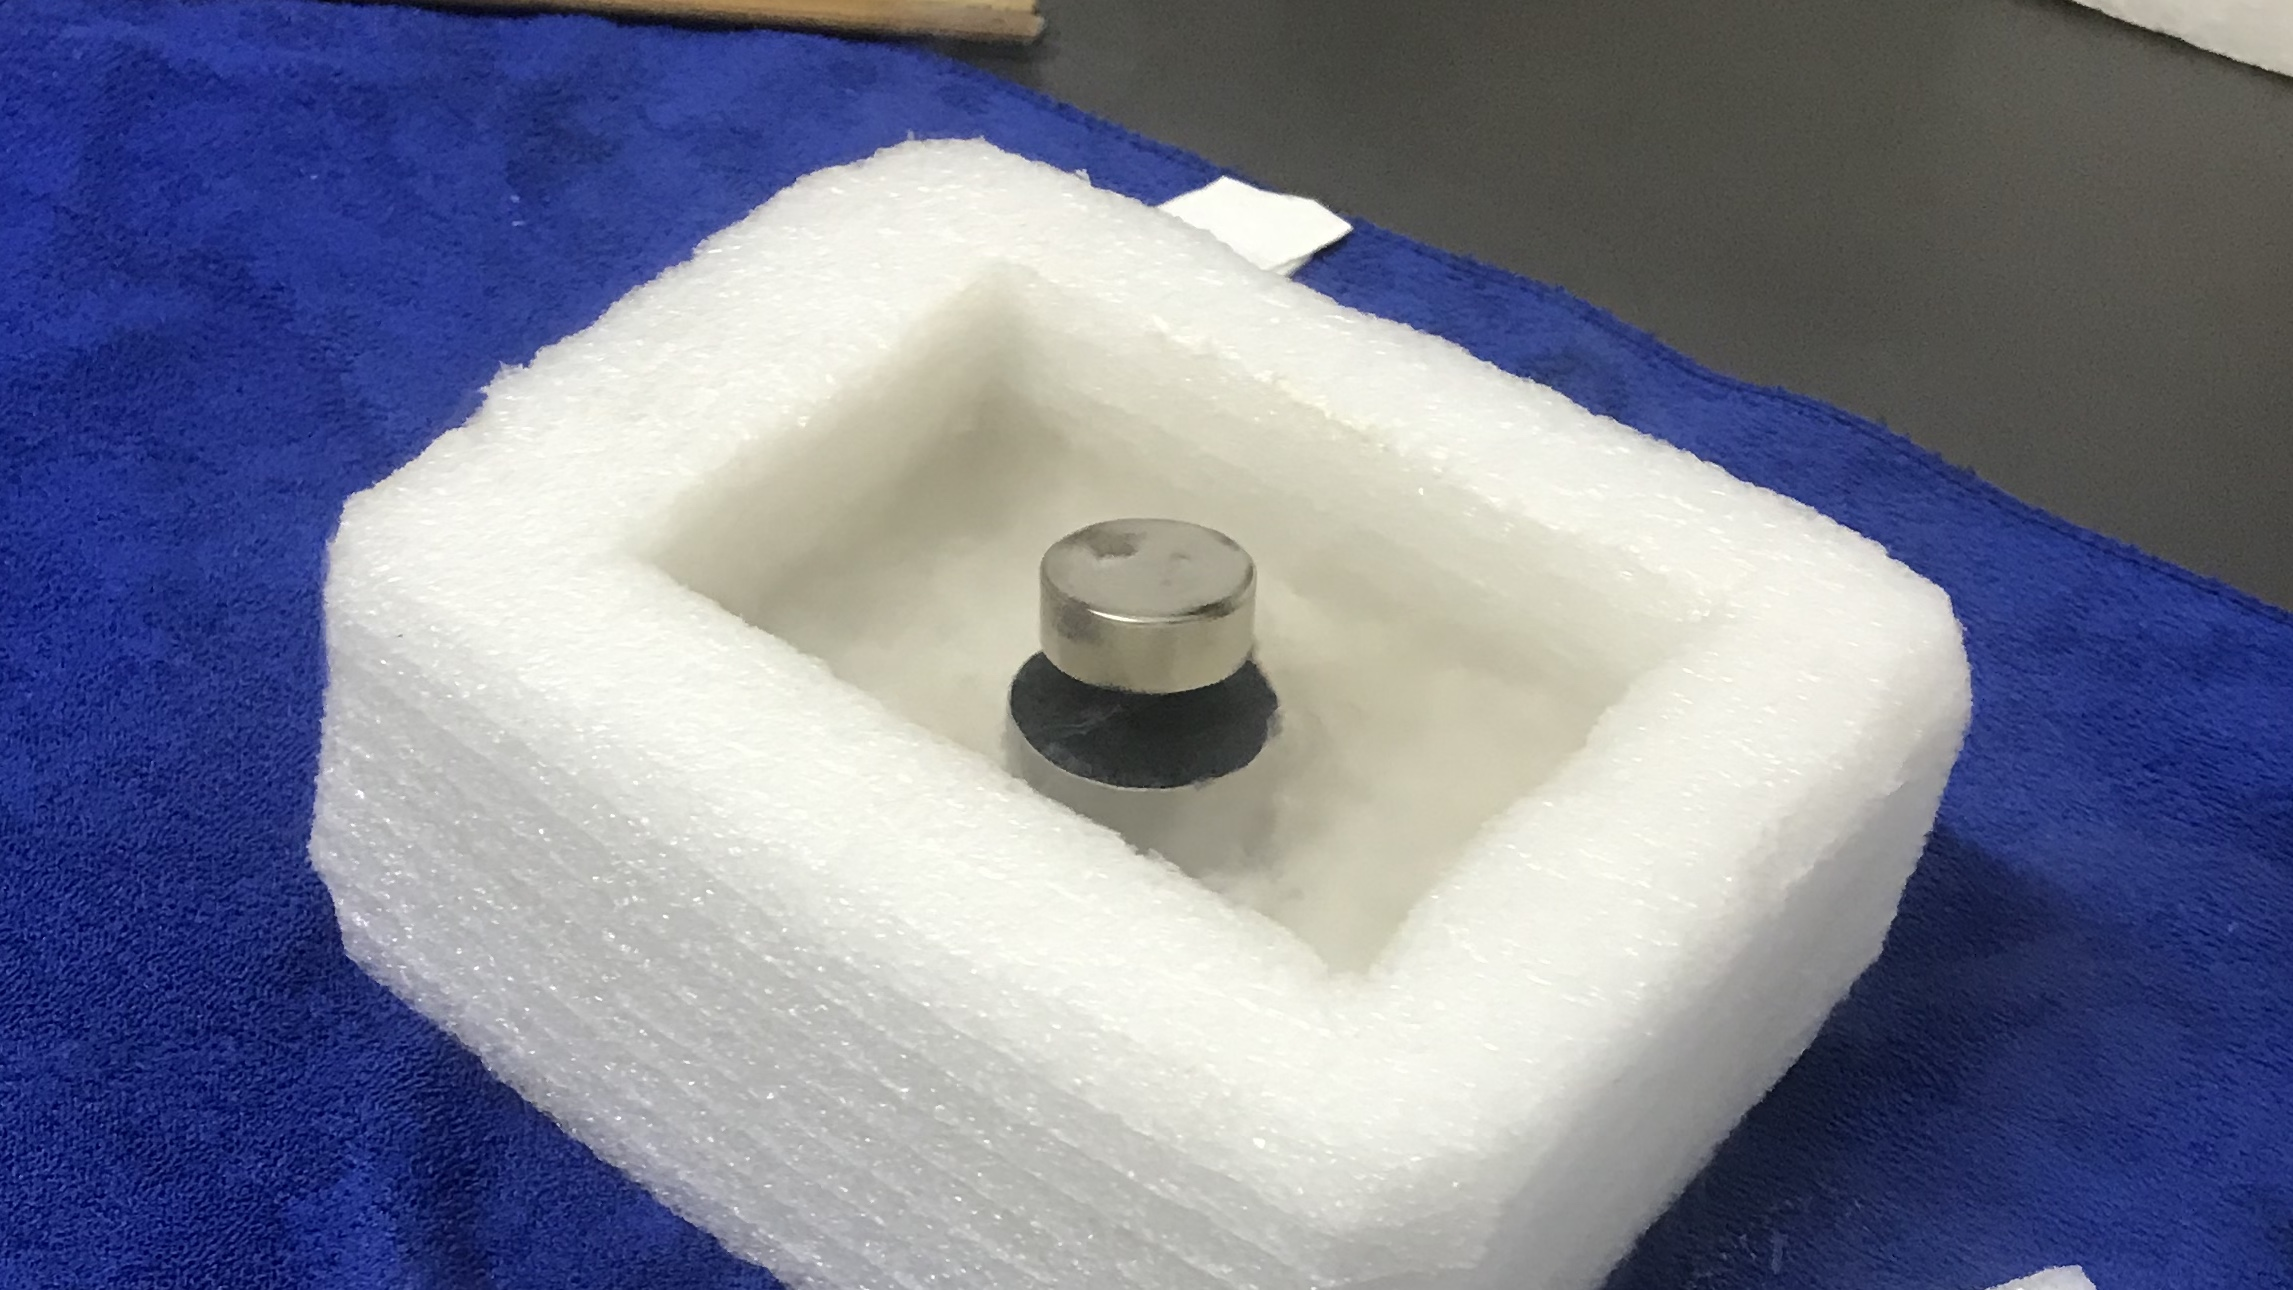
\includegraphics[width=6cm]{float.jpg}
\end{figure}
\begin{figure}[H]
\centering
  \subfigure[场冷条件]{ 
    \label{fig:subfig:a} %% label for first subfigure 
    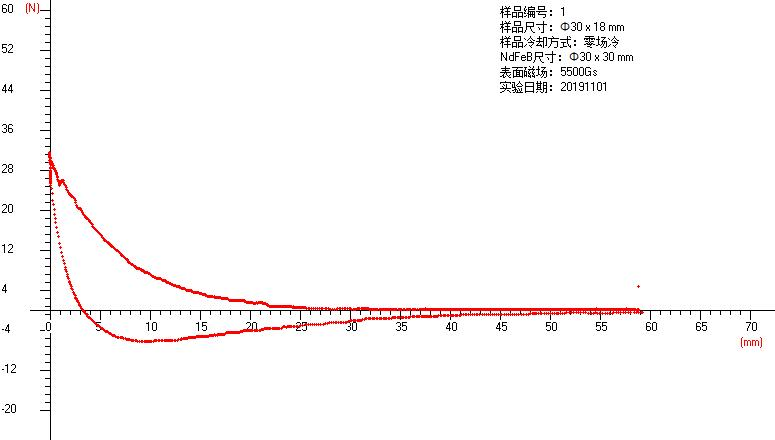
\includegraphics[width=7cm]{changleng.jpg}} 
  \subfigure[零场冷条件]{ 
    \label{fig:subfig:b} %% label for second subfigure 
    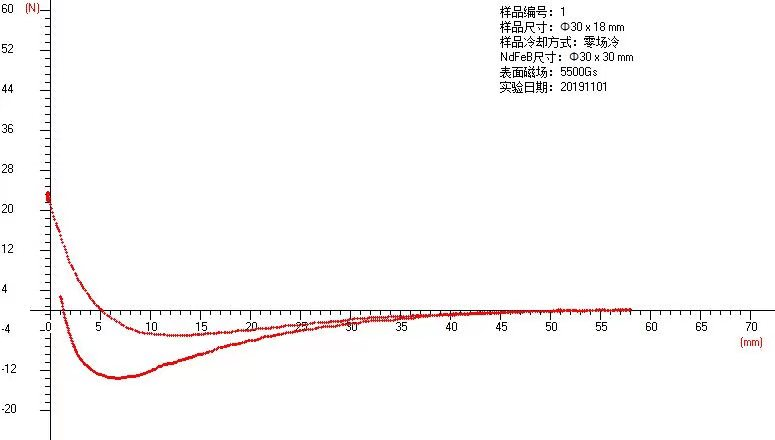
\includegraphics[width=7cm]{lingchangleng.jpg}} 
  \caption{高温超导体与磁铁间相互作用力;横轴:距离($mm$);纵轴:相互作用力($N$)} 
  \label{fig:subfig} %% label for entire figure 
\end{figure}
场冷条件下,上段曲线为磁铁与样品距离靠近时的曲线,下段曲线为磁铁与样品距离远离时的曲线。可见,当磁铁从最近处远离样品时,样品处于混合态,磁通线排出时受到阻力,表现为吸引力,吸引力随着距离增大而增大,但当磁通线排出较多后,吸引力开始减小,最后为0。当距离进一步减小时,磁通线进入受到阻力,表现为排斥力。 

零场冷条件下,其上段曲线为磁铁与样品距离靠近时的曲线,下段曲线远离时的曲线。可知当磁铁从最近处远离样品时,样品处于混合态,磁通线排出时会受到阻力,表现为吸引力,吸引力随着距离的增大而增大,但当磁通线排出较多时,吸引力不断减小,最后为0。

\section{误差分析}
测量R-T曲线时,温度较高时由于是手动记录的Pt电阻的电压和温差热电偶、样品、硅二极管的电压并不准确地对应,故存在一定的误差。

\section{结论}
超导体具有超导特性和完全抗磁性。在一定温度范围内,铂电阻、硅二极管以及温差电偶在电阻温度效应上都具有良好的线性关系,因此可以用作制作温度计。

\section{参考文献}
\small
\noindent[1]北师大物理实验教学中心,近代物理实验2讲义p23-45,2019.

\newpage
\begin{figure}[H]
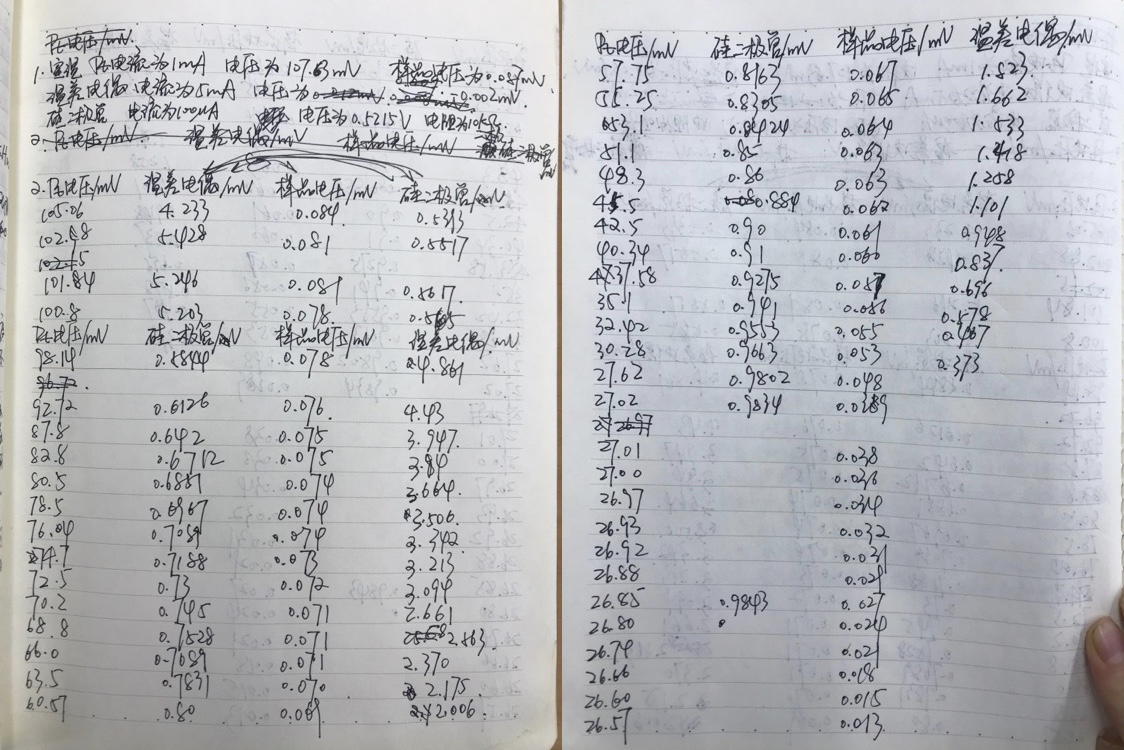
\includegraphics[width=15cm]{statistic1.jpg}
\end{figure}
\begin{figure}[H]
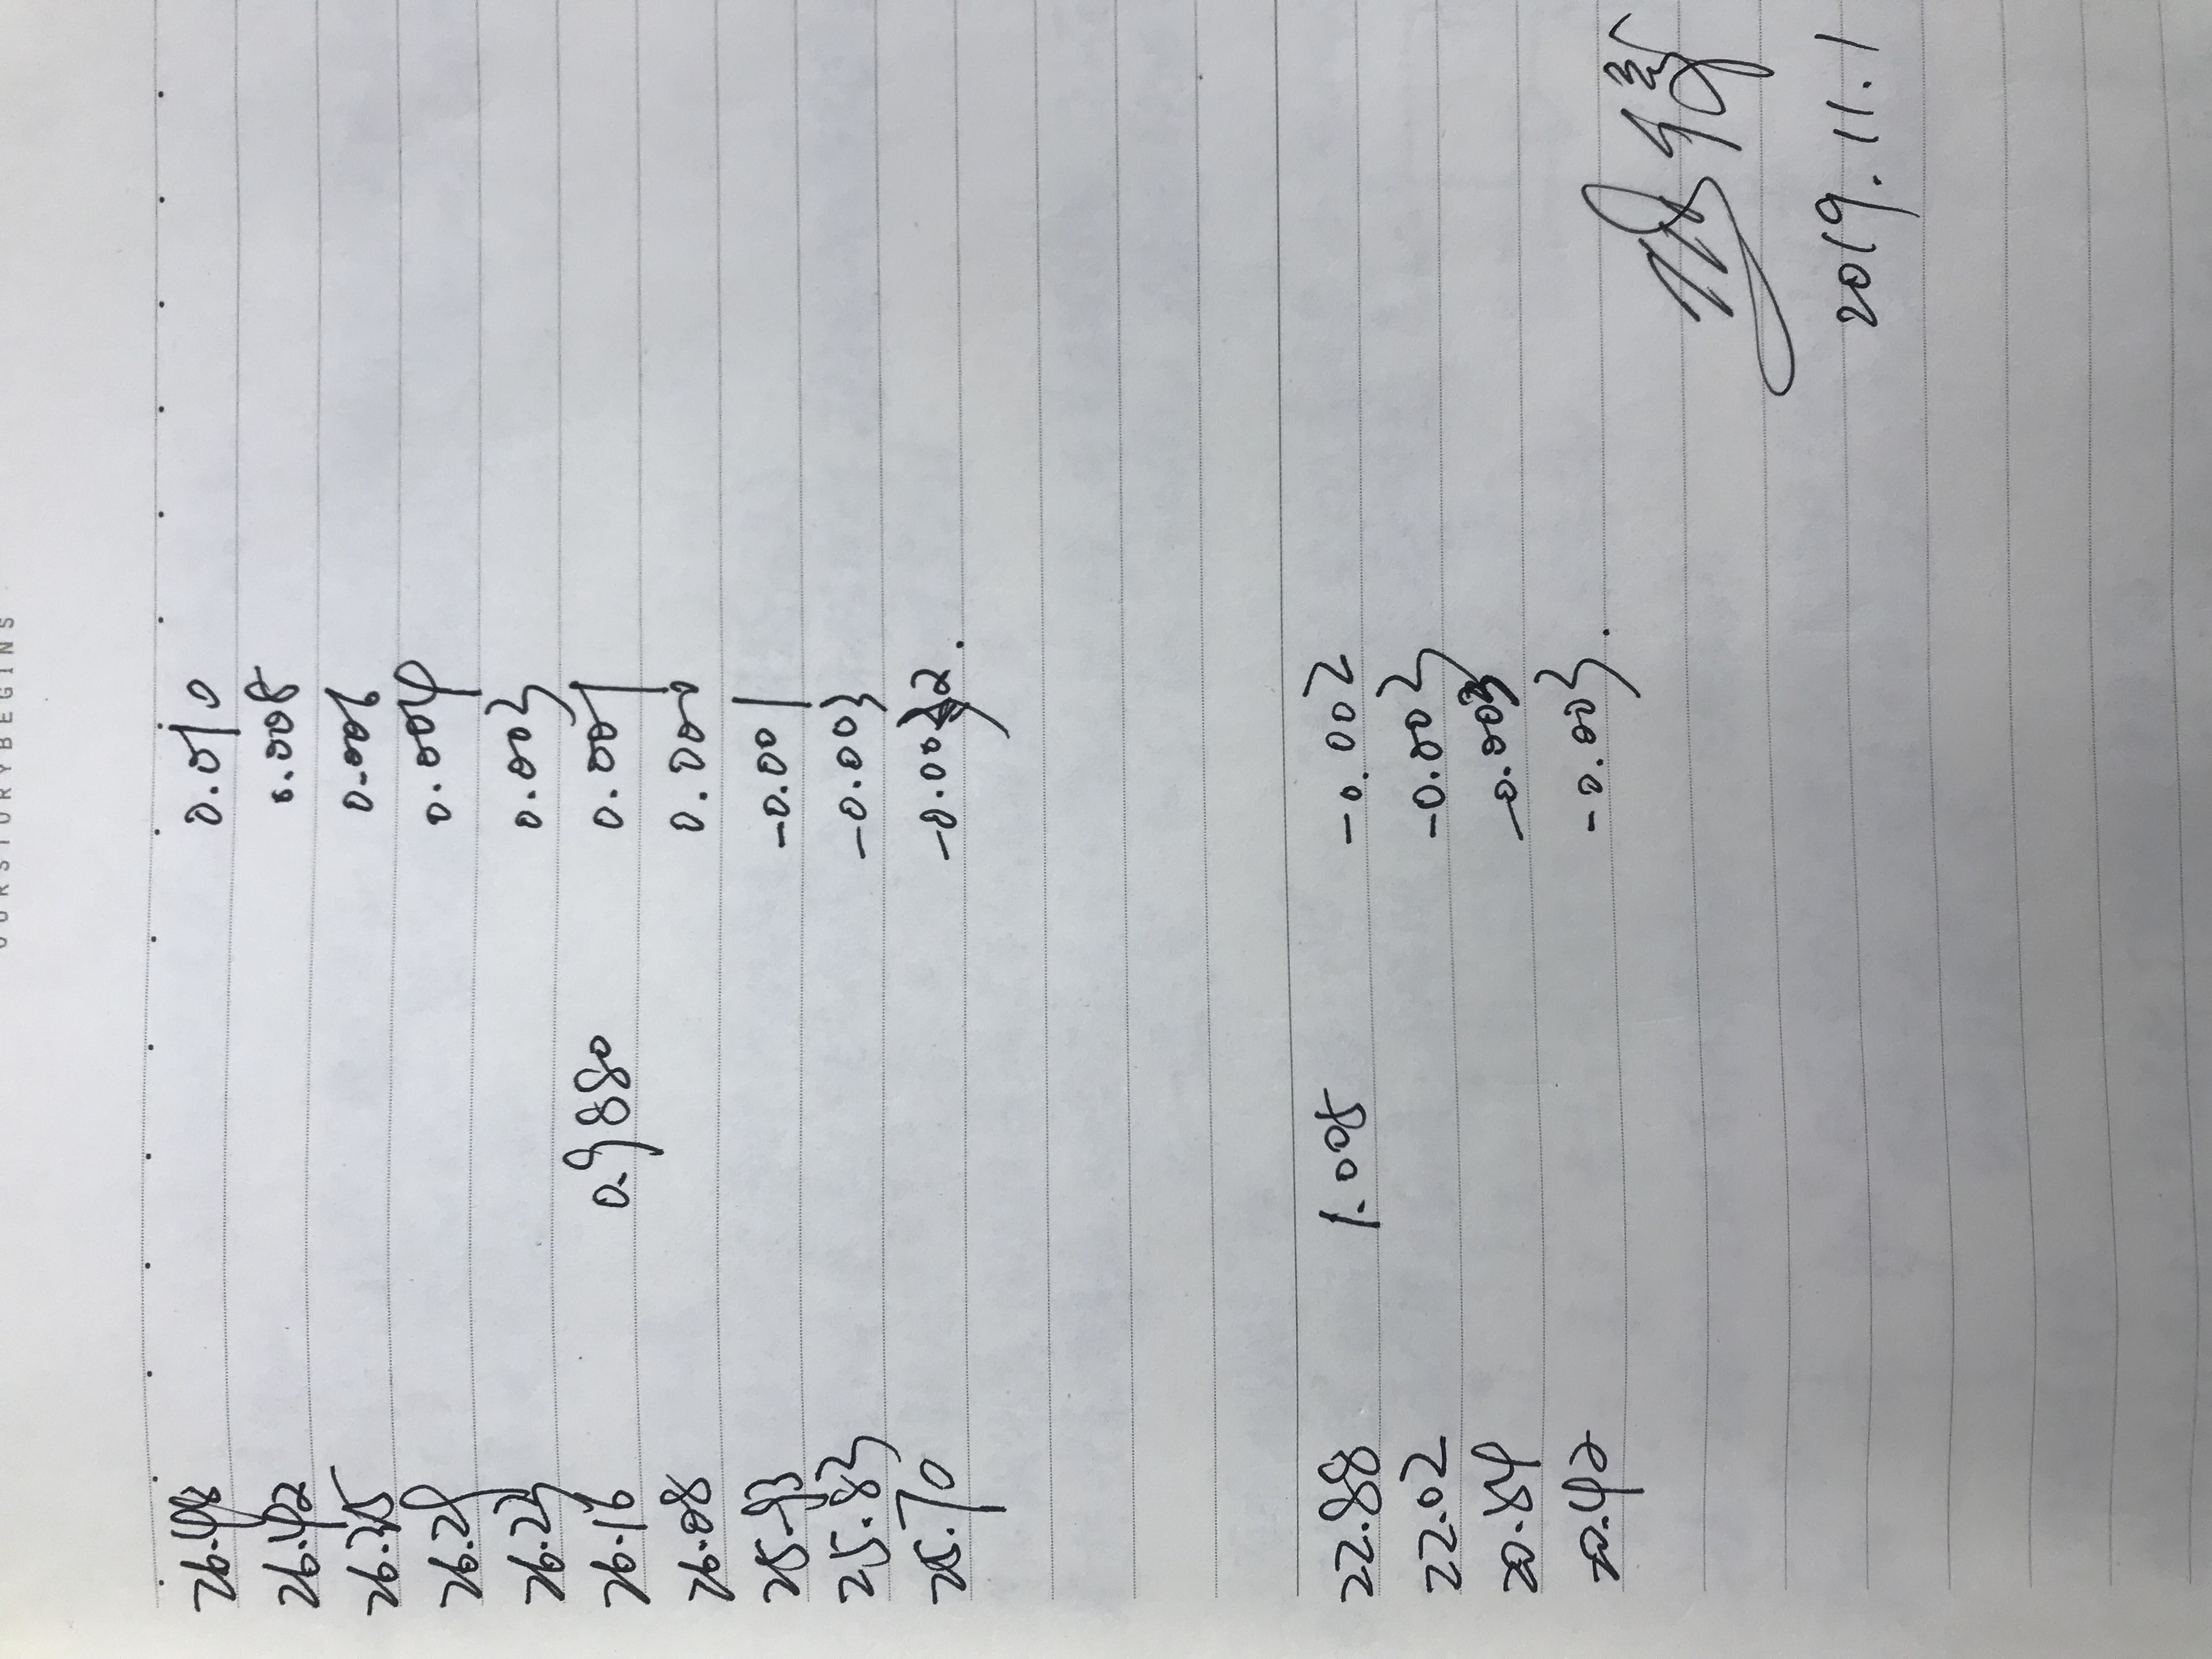
\includegraphics[width=10cm]{statistic3.jpg}
\end{figure}

\end{document}